% Chapter 2: The breadth-first walk
% Contains:
%   The definition of the breadth-first walk
%   The continuous version
%   The proof of Zn -> W

\chapter{The breadth-first walk} \label{C: bf-walk}
\fxnote{Update title.}

This chapter introduces the breadth-first walk, 
a way to traverse the vertices of a given graph such that component sizes can be read from the development of a \cadlag~process. 

\section{The breadth-first walk on a deterministic graph}
%%%%%%%%%%%%%%%%%%%%%%%%%%%%%%%%%%%%%%%%%%%%%%%%%%%%%%%%%%%%
% SECTION: The discrete breadth-first walk
%%%%%%%%%%%%%%%%%%%%%%%%%%%%%%%%%%%%%%%%%%%%%%%%%%%%%%%%%%%%

\subsection{In discrete time}
%%%%%%%%%%%%%%%%%%%%%%%%%%%%%%%%%%%%%%%%%%%%%%%%%%%%%%%%%%%%
% Introduction
%%%%%%%%%%%%%%%%%%%%%%%%%%%%%%%%%%%%%%%%%%%%%%%%%%%%%%%%%%%%
We start by describing the deterministic construction of this process.
Consider an arbitrary graph $\mathcal{G}$ on the set of vertices 
$V = \{1, \dots , n\} $ with set of edges $E$.
We will define the breadth-first ordering
$(v_1, \dots, v_n)$
of the vertices along with an integer-valued sequence
$(z(i), \; 1 \leq i \leq n)$
which we call the breadth-first walk on
$\mathcal{G}$.


%%%%%%%%%%%%%%%%%%%%%%%%%%%%%%%%%%%%%%%%%%%%%%%%%%%%%%%%%%%%
% Definition of breadth-first order
%%%%%%%%%%%%%%%%%%%%%%%%%%%%%%%%%%%%%%%%%%%%%%%%%%%%%%%%%%%%
The breadth-first order derives from an algorithmic construction as follows:
Let $\Ci{1}, \Ci{2}, \dots$ be the components of $\mathcal{G}$ in order, such that
$w_1, w_2, \dots$, the vertices with the smallest label in the corresponding component,
are ordered $w_1 > w_2 > \dots$. 
Call $w_i$ the root of $\Ci{i}$.
Now order by levels (distance from the root) and within levels order by original vertex label.
See Figure~\ref{F: bf-walk discrete} for an example of the new ordering.

For a more mathematically concise definition,
consider the set of vertices $\{ v_1,\dots, v_i \}$
and define the neighbour set $\Ni{i}$ as the vertices outside of
\fxnote{Add emphasis when needed}
$\{ v_1,\dots, v_i \}$ 
that are neighbours to some vertex in 
$\{ v_1,\dots, v_i \}$:
\begin{equation} \label{D: Ni}
\Ni{i} := 
\left\lbrace v \in V \backslash \{ v_1,\dots, v_i \} 
\; | \; 
\left(v_j, v\right) \in E \; \text{for some} \; 1 \leq j \leq i \right\rbrace
\end{equation}
This allows us to define the set of children of some vertex $v_i$ as
$\Ni{i} \backslash \Ni{i-1}$.
First order the components as described above. 
Now consider only the first component $\Ci{1}$.
Define $v_1 := w_1$, the root of $\Ci{1}$ and define
$v_2, \dots , v_{|\Ni{1}|+1}$ 
as the neighbours of $v_1$,
in increasing order of vertex label. 
Define the new label for all 
$i = 2, \dots, |\Ci{1}|$,
that is all vertices in the first component,
inductively by listing all children (if any exist) of $v_i$
in increasing order as 
$ v_{|\Ni{i-1}|+i}, \dots, v_{|\Ni{i}|+i} $.
After labelling the last vertex in $\Ci{1}$, set
$v_{|\Ci{1}| + 1} := w_2$, 
the root of $\Ci{2}$, and continue the construction as above.
Traverse all components this way.


%%%%%%%%%%%%%%%%%%%%%%%%%%%%%%%%%%%%%%%%%%%%%%%%%%%%%%%%%%%%
% Definitions of breadth-first walk
%%%%%%%%%%%%%%%%%%%%%%%%%%%%%%%%%%%%%%%%%%%%%%%%%%%%%%%%%%%%
For the number of children of $v_i$ write 
\begin{equation} \label{D: ci}
c(i) := |\Ni{i} \backslash\Ni{i-1}|.
\end{equation}
Now define the breadth-first walk 
$(z(i), \; 1 \leq i \leq n)$
by
\begin{equation} \label{E: def bf-walk z}
\begin{aligned}
z(0) &:= 0, \\
z(i) &:= z(i-1) + c(i) -1, \quad i=1, \dots , n.
\end{aligned}
\end{equation}


%%%%%%%%%%%%%%%%%%%%%%%%%%%%%%%%%%%%%%%%%%%%%%%%%%%%%%%%%%%%
% Explanation
%%%%%%%%%%%%%%%%%%%%%%%%%%%%%%%%%%%%%%%%%%%%%%%%%%%%%%%%%%%%

\begin{figure} [H]
	\centering
	\subfloat[Original vertex labels]
	{\begin{tikzpicture}[level distance = 11mm, scale = 1]
	\tikzstyle{level 1}=[sibling distance=8mm]
	\tikzstyle{level 2}=[sibling distance=8mm]
	\tikzstyle{level 3}=[sibling distance=8mm]
	
	\node [plain] (1) {1} [grow=up]
	child { node [plain] {\phantom{0}}
		child { node [plain] {\phantom{0}}
		}
		child { node [plain] {\phantom{0}}
		}
	}
	child { node [plain] {\phantom{0}}
	}
	;
	\node [plain] [right=2.5cm of 1] (6) {2} [grow=up]
	child { node [plain] {\phantom{0}}
		child { node [plain] {6}
		}
		child { node [plain] {\phantom{0}}
		}
		child { node [plain] {\phantom{0}}
		}
	}
	child { node [plain] (8) {\phantom{0}}
	}
	child { node [plain] {\phantom{0}}
		child { node [plain] (10) {\phantom{0}}
		}
	}
	;
	\node [plain] [right=2cm of 6] (14) {3} [grow=up]
	child { node [plain] {\phantom{0}}
	}
	;
	\node [plain] [right=1cm of 14] (16) {4} [grow=up]
	child { node [plain] {\phantom{0}}
	}
	child { node [plain] {\phantom{0}}
	}
	;
	\node [plain] [right=1cm of 16] (19) {5}
	;
	\node [plain] [right=1cm of 19] (20) {7} [grow=up]
	child { node [plain] {\phantom{0}}
	}
	child { node [plain] {\phantom{0}}
		child { node [plain] {\phantom{0}}
			child { node [plain] {\phantom{0}}
			}
			child { node [plain] {\phantom{0}}
			}
			child { node [plain] {\phantom{0}}
			}
			child { node [plain] {\phantom{0}}
			}
		}
	}
	;
	\draw (10) -- (8);
\end{tikzpicture}}\\
	
	\centering
	\subfloat[New vertex labels]
	{\begin{tikzpicture}[level distance = 11mm, scale = 1]
	\tikzstyle{level 1}=[sibling distance=8mm]
	\tikzstyle{level 2}=[sibling distance=8mm]
	\tikzstyle{level 3}=[sibling distance=8mm]
	
	\node [plain] (1) {$v_1$} [grow=up]
	child { node [plain] {$v_3$}
		child { node [plain] {$v_5$}
		}
		child { node [plain] {$v_4$}
		}
	}
	child { node [plain] {$v_2$}
	}
	;
	\node [plain] [right=2.5cm of 1] (6) {$v_6$} [grow=up]
	child { node [plain] {$v_9$}
		child { node [plain] {$v_{13}$}
		}
		child { node [plain] {$v_{12}$}
		}
		child { node [plain] {$v_{11}$}
		}
	}
	child { node [plain] (8) {$v_8$}
	}
	child { node [plain] {$v_7$}
		child { node [plain] (10) {$v_{10}$}
		}
	}
	;
	\node [plain] [right=2cm of 6] (14) {$v_{14}$} [grow=up]
	child { node [plain] {$v_{15}$}
	}
	;
	\node [plain] [right=1cm of 14] (16) {$v_{16}$} [grow=up]
	child { node [plain] {$v_{18}$}
	}
	child { node [plain] {$v_{17}$}
	}
	;
	\node [plain] [right=1cm of 16] (19) {$v_{19}$}
	;
	\node [plain] [right=1cm of 19] (20) {$v_{20}$} [grow=up]
	child { node [plain] {$v_{22}$}
	}
	child { node [plain] {$v_{21}$}
		child { node [plain] {$v_{23}$}
			child { node [plain] {$v_{27}$}
			}
			child { node [plain] {$v_{26}$}
			}
			child { node [plain] {$v_{25}$}
			}
			child { node [plain] {$v_{24}$}
			}
		}
	}
	;
	\draw (10) -- (8);
\end{tikzpicture}}\\
	
	\centering
	\subfloat[Resulting breadth-first walk, dashed lines indicating the end of components]
	{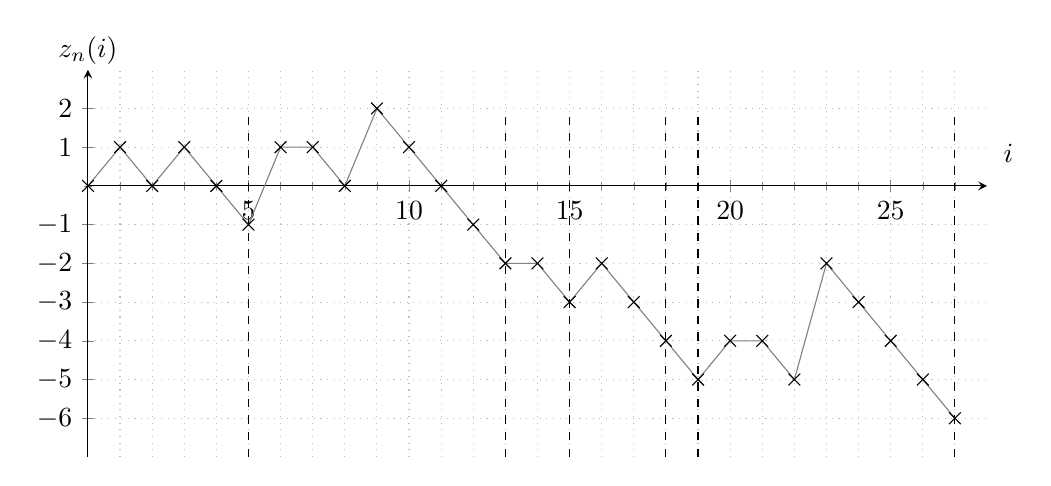
\begin{tikzpicture}

\begin{axis}[
axis x line=bottom,
axis y line=left,
grid = minor,
minor grid style={dotted},
xmin=0,
axis lines = middle,
xmax=28,
ymax = 3,
ymin  = -7,
xlabel={$i$},
x label style = {at={(axis description cs:1.04,0.785)},anchor=east},
ylabel={$z_n(i)$},
y label style = {at={(axis description cs:0,1.11)},anchor=north},
xtick={5,10,15,20,25},
minor xtick = {1,...,27},
ytick={-6,...,2},
minor ytick={-6,...,2},
width = 13cm,
height = 6.5cm
]

\addplot [
mark=x,
mark options={color=black, scale=1.5}, 
color=gray
]
coordinates{
	(0,0) (1,1) (2,0) (3,1) (4,0) (5,-1)
	(6,1) (7,1) (8,0) (9,2) (10,1) (11,0) (12,-1) (13,-2) 
	(14,-2) (15,-3) 
	(16,-2) (17,-3) (18,-4) 
	(19,-5) 
	(20, -4) (21,-4) (22,-5) (23,-2) (24,-3) (25,-4) (26, -5) (27,-6)
};


\addplot [dashed] coordinates {(5, -7) (5, 2)};
\addplot [dashed] coordinates {(13, -7) (13, 2)};
\addplot [dashed] coordinates {(15, -7) (15, 2)};
\addplot [dashed] coordinates {(18, -7) (18, 2)};
\addplot [dashed] coordinates {(19, -7) (19, 2)};
\addplot [dashed] coordinates {(27, -7) (27, 2)};
\end{axis}

\end{tikzpicture} }
	
	\caption{Breadth-first walk on the first components of a graph}
	\label{F: bf-walk discrete}
\end{figure} 

Figure~\ref{F: bf-walk discrete} shows this process for a graph example.
The root of each component is the vertex contained with the smallest original label.
Most other vertex labels are omitted since they do not play a role in the assignment of new labels.

The process divides the vertex set into three parts: 
Explored, discovered and neutral vertices. Every vertex starts as neutral.
At step $1$, we traverse vertex $1$ and mark it as explored with new label $v_1$.
We search for neighbours of $v_1$ and assign them labels to mark as discovered.
The next vertex to explore is the vertex already discovered with the smallest label
and each vertex switches from neutral to discovered once it gets assigned a new label.
Once we found all its neighbours, it switches to explored.
\fxnote{This whole paragraph}
After traversing every vertex of one component
there are no discovered vertices left and we continue the exploration with the neutral vertex with the smallest original label.

The walk $z$ decreases by $1$ for each vertex explored
and increases by the number of new neighbours discovered in each step.

Note that surplus edges, like $(v_8, v_{10})$ in Figure~\ref{F: bf-walk discrete}, are ignored by the breadth-first walk.
We count their occurrence with another counting process in Chapter~\ref{C: surplus edges}.





%%%%%%%%%%%%%%%%%%%%%%%%%%%%%%%%%%%%%%%%%%%%%%%%%%%%%%%%%%%%
% Equivalent definition
%%%%%%%%%%%%%%%%%%%%%%%%%%%%%%%%%%%%%%%%%%%%%%%%%%%%%%%%%%%%
We write
\begin{align}
\zeta(j) &:= |\Ci{1}| + \dots + |\Ci{j}|, \label{E: zeta}\\ 
\zeta^{-1}(i) &:= \min \{ j \; | \; \zeta(j) \geq i \}, \label{E: zeta-1}
\end{align}

for the index of the last vertex in the $j$-th component and the index of the component containing $v_i$,
respectively.
Now we can provide a definition of the breadth-first walk equivalent to \eqref{E: def bf-walk z}:
\begin{equation}  \label{E: def bf-walk z*}
\begin{aligned}
z^*(0) &:= 0, \\
z^*(i) &:= |\Ni{i}| - \zeta^{-1}(i), \quad i=1, \dots , n.
\end{aligned}
\end{equation}

We verify the equivalence by induction, showing that for $i \geq 2$ increments of both functions are equal.
We have
\begin{equation} \label{E: equality z z*}
\begin{aligned} 
&\hspace{35pt} z(i) - z(i-1) = z^*(i)  -z^*(i-1) \\
&\iff c(i) - 1 = |\Ni{i}| - \zeta^{-1}(i) - |\Ni{i-1}| + \zeta^{-1}(i-1) \\
&\iff |\Ni{i}| - |\Ni{i-1}| = c(i) + \zeta^{-1}(i) - \zeta^{-1}(i-1) - 1
\end{aligned}
\end{equation}
\fxnote{This equation does not look nice. Delete 1./2. row? Delete iffs?}
\fxnote{This has to hold for i >= 1, or fix the indices.}

We divide the proof into two cases.
First, assume $v_{i-1}$ is not the last vertex in its component.
Then $v_i$ belongs to the same component and
$\zeta^{-1}(i) = \zeta^{-1}(i-1)$.
Vertex $v_i$ has already been assigned a new label at step $i-1$,
so $v_i \in \Ni{i-1}$.
Going from $i-1$ to $i$,
the neighbour set increases by the number of new neighbours of $v_i$
and decreases by $v_i$ itself.
So
\begin{equation}
|\Ni{i}| - |\Ni{i-1}| = c(i) - 1,
\end{equation}
which provides the equality.

In the second case, if $v_{i-1}$ is the last vertex of its component,
then $\zeta^{-1}(i) = \zeta^{-1}(i-1) + 1$
and $|\Ni{i-1}| = 0$.
Equality \eqref{E: equality z z*} reduces to
$ |\Ni{i}| = c(i)$,
which holds since
$c(i) = |\Ni{i} \backslash \Ni{i-1}| = |\Ni{i}|$.
This proves the equivalence of both processes.
We proceed referring to the breadth-first walk as $z(i)$.

\bigskip

Since $|\Ni{i}| = 0$ only if $v_i$ is the last vertex in its component,
\eqref{E: zeta} and \eqref{E: def bf-walk z*} imply
\begin{equation} \label{E: (6).1}
	z(\zeta (j)) = -j
\end{equation}
and 
\begin{equation} \label{E: (6).2}
	z(i) \geq -j \quad \text{for all} \enspace \zeta(j) < i < \zeta(j+1).
\end{equation}

So, for vertices in the $j$-th component,
the random walk takes values greater or equal to $-(j-1)$,
until the last vertex, for which $z$ reaches a new minimum at $-j$.
Knowing this we can reconstruct sizes and indices of components via
\begin{align}
\zeta(j) &= \min \{ i \; | \; z(i) = -j \}, \label{E: zeta(j) = min(i)} \\
|\Ci{j}| &= \zeta(j) - \zeta(j-1), \label{E: C(j) = zeta - zeta} \\
\zeta^{-1}(i) &= 1 - \min_{j \leq i-1}z(j). \label{E: zeta-1(i) = 1 - min(j)}
\end{align}
\fxnote{Maybe add some more explanation on where these formulas come from.}


\subsection{In continuous time}
%%%%%%%%%%%%%%%%%%%%%%%%%%%%%%%%%%%%%%%%%%%%%%%%%%%%%%%%%%%%
% SECTION: The continuous-time breadth-first walk
%%%%%%%%%%%%%%%%%%%%%%%%%%%%%%%%%%%%%%%%%%%%%%%%%%%%%%%%%%%%

The last section defined the random walk for integer times,
but to develop our theory of convergence to a Brownian motion
we will have to construct $z(i)$ in continuous time.

Define a sequence of independent random variables, 
uniformly distributed on $(0,1)$, 
$(\Uij, 1 \leq i \leq n, 1 \leq j \leq c(i))$,
where $c(i)$ is the number of children of $v_i$.

Then for each $i = 1, \dots, n$ and $0 \leq u \leq 1$ define the process $Z$ by
\begin{equation} \label{E: def Z}
\begin{aligned}
Z(0) &:= 0, \\
Z(i - 1 + u) &:= Z(i-1) - u + \sum_{1 \leq j \leq c(i)} \Ind{\{ \Uij \leq u \}}.
\end{aligned}
\end{equation}
So $Z(i) = Z(i-1) - 1 + c(i)$ and $Z$ coincides with the discrete definition of the breadth-first walk at integer times.

Some more explanation on this construction:
At time $i-1$, 
the walk has traversed vertices
$(v_1, \dots, v_{i-1})$
and has discovered a list of vertices
$(v_1, \dots, v_k)$
of length
$k = i-1 + |\Ni{i-1}|$.
The discrete walk now adds the children of $v_i$ to this list at time $i$.
The newly defined continuous walk adds those vertices at uniformly random times in $(i-1, i)$.

\begin{figure}[H]
	\centering
	\subfloat[A graph component]
	{\begin{tikzpicture}[level distance = 11mm, scale = 1]
	\tikzstyle{level 1}=[sibling distance=10mm]
	\tikzstyle{level 2}=[sibling distance=8mm]
	
	\node [plain] [right=2.5cm of 1] (1) {$v_1$} [grow=up]
	child { node [plain] {$v_4$}
		child { node [plain] {$v_8$}
		}
		child { node [plain] {$v_7$}
		}
		child { node [plain] {$v_6$}
		}
	}
	child { node [plain] (3) {$v_3$}
	}
	child { node [plain] {$v_2$}
		child { node [plain] (5) {$v_5$}
		}
	}
	;
\end{tikzpicture}}\\
	
	\centering
	\subfloat[The continuous-time breadth-first walk]
	{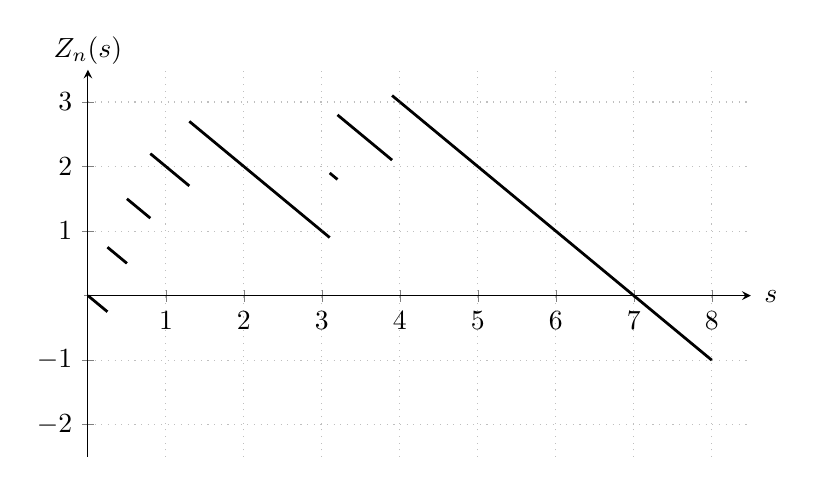
\begin{tikzpicture}

\begin{axis}[
axis x line=bottom,
axis y line=left,
grid = minor,
minor grid style={dotted},
xmin=0,
axis lines = middle,
xmax=8.5,
ymax = 3.5,
ymin  = -2.5,
xlabel={$s$},
x label style = {at={(axis description cs:1.055,0.415)},anchor=east},
ylabel={$Z_n(s)$},
y label style = {at={(axis description cs:0,1.11)},anchor=north},
xtick={1,...,8},
minor xtick = {1,...,8},
ytick={-2,...,3},
minor ytick={-2,...,3},
width = 10cm,
height = 6.5cm
]

%\addplot [
%line width=1.0pt
%]
%coordinates{
%	(0,0) (0.25,-0.25) (0.25,0.75) (0.5,0.5) (0.5,1.5) (0.8,1.2) (0.8,2.2) (1,2)
%	(1.3, 1.7) (1.3, 2.7) (2,2)
%	(3,1)
%	(3.1, 0.9) (3.1,1.9) (3.2,1.8) (3.2,2.8) (3.9,2.1) (3.9,3.1) (4,3)
%	(5,2) (6,1) (7,0) (8,-1)
%};

\addplot [line width=1.0pt]coordinates{(0,0) (0.25,-0.25)};
\addplot [line width=1.0pt]coordinates{(0.25,0.75) (0.5,0.5)};
\addplot [line width=1.0pt]coordinates{(0.5,1.5) (0.8,1.2)};
\addplot [line width=1.0pt]coordinates{(0.8,2.2) (1,2)};
\addplot [line width=1.0pt]coordinates{(1,2) (1.3, 1.7)};
\addplot [line width=1.0pt]coordinates{(1.3, 2.7) (2,2)};
\addplot [line width=1.0pt]coordinates{};
\addplot [line width=1.0pt]coordinates{(2,2) (3,1)};
\addplot [line width=1.0pt]coordinates{(3,1) (3.1, 0.9)};
\addplot [line width=1.0pt]coordinates{(3.1,1.9) (3.2,1.8)};
\addplot [line width=1.0pt]coordinates{(3.2,2.8) (3.9,2.1)};
\addplot [line width=1.0pt]coordinates{(3.9,3.1) (4,3)};
\addplot [line width=1.0pt]coordinates{(4,3) (8,-1)};

%% Dashed lines indicate end of vertex, but the xick already do that
%\addplot [dashed] coordinates {(1, -2.5) (1, 3.5)};
%\addplot [dashed] coordinates {(2, -2.5) (2, 3.5)};
%\addplot [dashed] coordinates {(3, -2.5) (3, 3.5)};
%\addplot [dashed] coordinates {(4, -2.5) (4, 3.5)};
%\addplot [dashed] coordinates {(5, -2.5) (5, 3.5)};
%\addplot [dashed] coordinates {(6, -2.5) (6, 3.5)};
%\addplot [dashed] coordinates {(7, -2.5) (7, 3.5)};
%\addplot [dashed] coordinates {(8, -2.5) (8, 3.5)};

\end{axis}

\end{tikzpicture} }
	
	\caption{Continuous breadth-first walk on a single component}
	\label{F: bf-walk cont}
\end{figure} 

Note that, 
since jumps are now happening at random times during their respective time interval, 
$Z$ is a stochastic process even though it is still only defined for a given deterministic graph.


\section{The breadth-first walk as a stochastic process}
%%%%%%%%%%%%%%%%%%%%%%%%%%%%%%%%%%%%%%%%%%%%%%%%%%%%%%%%%%%%
% SECTION: The central limit theorem for martingales
%%%%%%%%%%%%%%%%%%%%%%%%%%%%%%%%%%%%%%%%%%%%%%%%%%%%%%%%%%%%
\fxfatal{Update title}

Denote by $Z_{\Gcal}$ the continuous-time breadth-first walk on the graph $\Gcal$
and define
\begin{equation} \label{D: znt}
	\znt(\omega, s) := Z_{\Gcal^{\pp}(\omega)}(s)
\end{equation}
where $\Gcal^{\pp}(\omega)$ is a realization of the critical random graph $\Gnt$.
We can now state the main theorem of this chapter,
the convergence in distribution of this process to a Brownian motion with drift after rescaling.

\begin{theorem} \label{T: Z -> W}
	Let $\znt(s)$, for $0 \leq s \leq n$, 
	be the breadth-first walk associated with $\Gnt$.
	Rescale via
	\begin{equation}
	\rznt(s) := \n{-1}{3} \znt(\n{2}{3}s).
	\end{equation}
	Then $\rznt(s) \rightarrow_d \Wt$ as $n \rightarrow \infty$.
\end{theorem}


\subsection{Decompositions of $\znt$}
%%%%%%%%%%%%%%%%%%%%%%%%%%%%%%%%%%%%%%%%%%%%%%%%%%%%%%%%%%%%
% SECTION: Decompositions of $\Zn$
%%%%%%%%%%%%%%%%%%%%%%%%%%%%%%%%%%%%%%%%%%%%%%%%%%%%%%%%%%%%

In the next sections we prove Theorem~\ref{T: Z -> W}.
We begin by providing a suitable decomposition of $\znt$ into a martingale and
an integrable predictable process.
The latter process will later provide the downwards drift of $\Wt$,
while we go on proving the convergence of the martingale to a standard Brownian motion.

Since $\Zn$ increases by $1$ for every event of a new edge appearing in the breadth-first walk
we may view the process as a Poisson point process on the positive real line with a certain constant downwards drift.
This point process would then possess a conditional intensity, say $\an(s)$, such that
\begin{equation}
	\an(s)ds = \Exp{ \Zn(s + ds) - \Zn(s) + ds \cond \F{s} }.
\end{equation}
We evaluate these considerations more elaborately in the following lemma.
For ease of notation we drop the superscript $\pp$ from all random variables in this chapter.

\begin{lemma} \label{L: decomp Zn}
	The decomposition 
	\begin{equation} \label{E: decomp Zn}
	\Zn = \Mn + \An
	\end{equation}
	holds, where $\Mn$ is a martingale and $\An$ is defined by
	\begin{equation} \label{D: An}
	\An(t) := \int_{0}^{t} a_n(s)ds - t
	\end{equation}
	with
	\begin{equation} \label{D: an}
	a_n(s)ds = \Prob(\text{A new edge appears in} \enspace [s, s+ds] \cond \Zn(u), \enspace u \leq s).
	\end{equation}
\end{lemma}

%%%%%%%%%%%%%%%%%%%%%%%%%%%%%%%%%%%%%%%%%%%%%%%%%%%%%%%%%%%%
% Lemma Decompositions An: Proof
%%%%%%%%%%%%%%%%%%%%%%%%%%%%%%%%%%%%%%%%%%%%%%%%%%%%%%%%%%%%
\begin{proof} \label{P: decomp Zn}
	We will prove that $\Zn - \An$ is a martingale by showing that
	\begin{equation} \label{E: Mn martingale}
	\Exp{ \Zn(t+u) - \An(t+u) \cond \F{t} } = \Zn(t) - \An(t)
	\end{equation}
	holds for all $u \geq 0$, where $\F{t}$ is the natural $\sigma$-algebra generated by $\Zn$, 
	$\F{t} = \sigma(\Zn(s), s \leq t).$
	This is equivalent to 
	\begin{equation}
	\Exp{\Zn(t+u) - \Zn(t) \cond \F{t}} = \Exp{\An(t+u) - \An(t) \cond \F{t}}.
	\end{equation}
	
	We start with the left-hand side. 
	The change of $\Zn$ between times $t$ and $t+u$ is the sum of all jumps that occurred in $[t, t+u]$,
	minus the constant downward drift $u$:
	\begin{align*}
	&\Exp{\Zn(t+u) - \Zn(t) \cond \F{t}} \\
	&\quad= \Exp{\text{Number of jumps in} \enspace [t, t+u] \cond \F{t}} - u \\
	&\quad= \Exp{\text{Number of new edges appearing in} \enspace [t, t+u] \cond \F{t}} - u,
	\end{align*}
	since every new edge corresponds to a jump of size $1$ in $\Zn$.
	
	Looking at the right-hand side, we define $\NewEdge{I}$ as the event of a new edge appearing during the time interval $I$ and calculate
	\begin{align*}
	&\Exp{\An(t+u) - \An(t) \cond \F{t}} \\
	&\quad= \Exp{ \int_{0}^{t+u} a_n(s)ds - (t+u) - \int_{0}^{t} a_n(s)ds + t \cond \F{t} } \\
	&\quad= \Exp{ \int_{t}^{t+u} a_n(s)ds \cond \F{t} } - u \\
	&\quad= \int_{t}^{t+u} \Exp{a_n(s)ds \cond \F{t}} - u \\
	&\quad= \int_{t}^{t+u} \Exp{ \Prob(\NewEdge{\sds} \cond \F{s}) \cond \F{t} } - u\\
	&\quad= \int_{t}^{t+u} \Prob( \NewEdge{\sds} \cond \F{t} ) - u
	\quad \text{since} \enspace \F{t} \subseteq \F{s} \enspace \forall s \in [t,t+u] \\
	&\quad= \Exp{ \int_{t}^{t+u}  \Ind{\NewEdge{\sds}} \cond \F{t}} -u \\
	&\quad= \Exp{\text{Number of new edges appearing in} \enspace [t, t+u] \cond \F{t}} - u.
	\end{align*}
	
	
	This proves $\Mn$ to be a martingale. 	
\end{proof}

For a better understanding of the processes involved, we need to find a concise expression for the probability used in \eqref{D: an}.
An ensuing corollary provides some characteristics of the resulting process $\An$.
Denote by $\floor{s}$ and $\ceil{s}$ the largest integer smaller than $s$ and the smallest integer larger than $s$, respectively.
Since the original vertex labels are no longer relevant,
we use the notion of vertex $v_i$ and vertex $i$ interchangeably.
\fxnote{See if this clarification is needed.}
We denote an edge between $v_i$ and $v_j$ by $(i,j)$.

%%%%%%%%%%%%%%%%%%%%%%%%%%%%%%%%%%%%%%%%%%%%%%%%%%%%%%%%%%%%
% Lemma Formula An: Statement
%%%%%%%%%%%%%%%%%%%%%%%%%%%%%%%%%%%%%%%%%%%%%%%%%%%%%%%%%%%%
\begin{lemma} \label{L: formula an}
	For $a_n$ as defined in Lemma~\ref{L: decomp Zn}, we have
	\begin{equation}
	\an(s) = (n - s - \Zetan{\ceil{s}} - \Zn(s)) \ps .
	\end{equation}
\end{lemma}

%%%%%%%%%%%%%%%%%%%%%%%%%%%%%%%%%%%%%%%%%%%%%%%%%%%%%%%%%%%%
% Lemma Formula An: Proof
%%%%%%%%%%%%%%%%%%%%%%%%%%%%%%%%%%%%%%%%%%%%%%%%%%%%%%%%%%%%
\begin{proof} \label{P: formula an}
	Consider the walk $\Zn$ at time $s\in[i-1, i]$.
	Let $N$ be the number of vertices that, at time $i-1$, were eligible to be children of vertex $v_i$.
	That is the number of vertices not yet explored or discovered, which excludes $v_i$ itself in particular.
	To any eligible vertex $v_j$ we assign a random variable $\Uij$.
	Let all $\Uij$ be independent and identically $\mathcal{U}(0,1)$ distributed.
	Our understanding of the process of discovering children of $v_i$ is as follows:
	At time $i-1+\Uij$, the edge $(i,j)$ will open with probability $\p$ and
	$\Zn$ will make a jump of size $1$.
	We arrive at a characterisation of our breadth-first walk, 
	equivalent to \eqref{E: def Z}:	
	\begin{equation}
	\Zn(i-1+u) = \Zn(i-1) - u + \sum_{j=1}^{N} \Ind{\{\Uij \leq u, \; (i,j) \; \text{open}\}}.
	\end{equation}
	
	We define $\SigmaAlgebra_s := \sigma(\Zn(u), u\leq s)$.
	The goal of this proof is to find an expression for
	$\Prob(\text{A new edge appears in $[s, s+ds]$} \cond \SigmaAlgebra_s)$.
	To do this, we condition over a finer $\sigma$-algebra and use the law of total expectation to arrive at a general statement.
	$\SigmaAlgebra_s$ tells us the history of the walk until time $s$. 
	We know how many vertices were eligible at time $i-1$ and how many open edges to $v_i$ were found in $[\floor{s},s]$.
	However, it is unknown exactly which vertices are now children of $v_i$ and which vertices are still eligible.
	Define 
	\begin{equation}
	\begin{split}
	\SigmaAlgebra_s^k := \sigma(&\Zn(u), u\leq s; \\
	&\text{There are exactly $k$ children of $v_i$ encountered thus far}, \\
	&\text{and these are $j_1, \dots, j_k$}).
	\end{split}
	\end{equation}
	
	We know that $k$ of the $N$ edges eligible at time $i-1$ are already open 
	and want to calculate the probability that one of the remaining $N-k$ edges opens in $[s, s+ds]$.
	The probability of some edge opening is the sum of the probabilities for single edges opening
	and some factor describing the, for small $ds$ increasingly slim, 
	chance of two or more edges opening in the interval.
	We denote by $\NewEdge{I}$ the event of a new edge appearing in an interval $I$ and write
	\begin{equation}
	\Prob(\NewEdge{[s,s+ds]} \cond \SigmaAlgebra_s^k)
	= \sum_{j \neq j_1, \dots j_k} \Prob( \text{$(i,j)$ opens in $[s, s+ds]$} \cond \SigmaAlgebra_s^k ) + \Smallo{ds}.
	\end{equation}
	For the edge $(i,j)$, all relevant information contained in $\SigmaAlgebra_s^k$ is the fact that 
	$(i,j)$ is not yet open, the event of opening has not happened in $[\floor{s}, s)$.
	Since the opening itself, happening with probability $\p$,
	and the uniformly distributed time of the event in $[i-1, i]$ are independent,
	we see that
	\begin{equation}
	\begin{aligned}
	&\Prob(\text{$(i,j)$ opens in $[s, s+ds]$}) \\
	&\quad = \Prob(\text{$(i,j)$ opens})\Prob(\text{It happens in $[s, s+ds]$}) \\
	&\quad = \p ds.
	\end{aligned}
	\end{equation}
	By the definition of conditional probability
	\begin{equation}
	\begin{aligned}
	&\Prob( \text{$(i,j)$ opens in $[s, s+ds]$} \cond \text{$(i,j)$ did not open in $[\floor{s}, s]$} ) \\
	&\quad = \frac{\Prob( \text{$(i,j)$ opens in $[s, s+ds]$})}{\Prob(\text{$(i,j)$ did not open in $[\floor{s}, s]$})} \\
	&\quad = \frac{\p ds}{1-\p(s-\floor{s})},
	\end{aligned}
	\end{equation}
	and finally, omitting the $\Smallo{ds}$-term, we have
	\begin{equation}
	\begin{aligned}
	\Prob(\NewEdge{[s,s+ds]} \cond \SigmaAlgebra_s^k) 
	&= \sum_{j \neq j_1, \dots j_k} \ps \\
	&= (N-k) \frac{\p ds}{1-\p(s-\floor{s})}.
	\end{aligned}
	\end{equation}
	Seeing that $\SigmaAlgebra_s \subseteq \SigmaAlgebra_s^k$,
	we apply the tower property:
	\begin{equation}
	\begin{aligned}
	\Prob(\NewEdge{[s,s+ds]} \cond \SigmaAlgebra_s)
	&= \Exp{\Ind{\NewEdge{[s,s+ds]}} \cond \SigmaAlgebra_s} \\
	&= \Exp{ \Exp{\Ind{\NewEdge{[s,s+ds]}} \cond \SigmaAlgebra_s^k} \cond \SigmaAlgebra_s} \\
	&= \Exp{ (N-k) \ps ds \cond \SigmaAlgebra_s}.
	\end{aligned}
	\end{equation}
	Conditioning on $\SigmaAlgebra_s$,
	the breadth-first walk $\Zn$ tells us exactly how many vertices have connected to vertex $v_i$ until time $s$.
	We denote by $\Ineligible{s}$ the number of vertices that are at time $s$ not eligible to be a child of $v(\ceil{s})$. \label{I: eta}
	Then $N-k=n-\Ineligible{s}$ at time $s$ and
	\begin{equation}
	\an(s)ds = \Prob(\NewEdge{\sds} \cond \SigmaAlgebra_s) = (n - \Ineligible{s}) \ps ds.
	\end{equation}
	
	\bigskip
	
	Finally, we find a concise expression for $\Ineligible{s}$.
	At time $i-1$, the ineligible vertices are the $i-1$ vertices already explored
	and the set $\Ni{i-1}$ of vertices already discovered as children.
	If $v_{i-1}$ is the last vertex of its component,
	$v_i$ itself is not part of $\Ni{i-1}$, 
	so we need to add a term that equals $1$ if $v_{i-1}$ is the last vertex of its component and $0$ otherwise.
	Together, we arrive at
	\begin{equation}
	\Ineligible{i-1} = i-1 + |\Ni{i-1}| + (\ZetaMinus{i} - \ZetaMinus{i-1}).
	\end{equation}
	By \eqref{E: def bf-walk z*} this is equivalent to
	\begin{equation}
	\Ineligible{i-1} = i-1 + \ZetaMinus{i} + \Zn(i-1).
	\end{equation}
	At time $i-1+u$, for $0<u<1$, 
	new vertices were discovered as children of $v_i$ and now add to $\Ineligible{i-1+u}$.
	The number of ineligible vertices is now
	\begin{equation}
	\begin{aligned}
	\Ineligible{i-1+u} 
	&= i-1 + \ZetaMinus{i} + \Zn(i-1) + \sum_{j} \Ind{\Uij \leq u} \\
	&= i-1+u + \ZetaMinus{i} + \Zn(i-1+u),
	\end{aligned}
	\end{equation} 
	by the definition of the continuous-time breadth-first walk in \eqref{E: def Z}.
	So $\Ineligible{s} = s + \ZetaMinus{\ceil{s}} + \Zn(s)$ which concludes the proof.
\end{proof}

%%%%%%%%%%%%%%%%%%%%%%%%%%%%%%%%%%%%%%%%%%%%%%%%%%%%%%%%%%%%
% Corollary An BV: Statement
%%%%%%%%%%%%%%%%%%%%%%%%%%%%%%%%%%%%%%%%%%%%%%%%%%%%%%%%%%%%
\begin{corollary}
	The process $\An$, as defined in Lemma~\ref{L: decomp Zn}, is a continuous process of bounded variation.
	Moreover, $\Zn$ and $\Mn$ are \cadlag~processes of bounded variation.
\end{corollary}

%%%%%%%%%%%%%%%%%%%%%%%%%%%%%%%%%%%%%%%%%%%%%%%%%%%%%%%%%%%%
% Corollary An BV: Proof
%%%%%%%%%%%%%%%%%%%%%%%%%%%%%%%%%%%%%%%%%%%%%%%%%%%%%%%%%%%%
\begin{proof}
	Since $\an(s) = (n - \Ineligible{s}) \ps \geq 0$ for all $s$,
	the integral $\int_{0}^{t}\an(s)ds$ is a non-decreasing, continuous function in $t$.
	Therefore $\An(t) = \int_{0}^{t}\an(s)ds -t$ is the difference of two continuous, non-decreasing functions.
	By the Jordan Decomposition, see e.g. \cite[Proposition 22, p.236]{Royden.1969}, $\An$ is a continuous process of bounded variation.
	
	We remember from the definition of the continuous-time breadth-first walk in $\eqref{E: def Z}$
	that $\Zn$ is the sum of the constant downward stream and jumps of size $1$ for every new edge.
	By the Jordan Decomposition, $\Zn$ is of bounded variation and the jumps make it a \cadlag~process.
	Since $\Mn = \Zn - \An$ is the difference of two functions of bounded variation, 
	it is again of bounded variation.
	Since $\An$ is continuous and $\Zn$ is \cadlag, $\Mn$ is \cadlag.
\end{proof}


%%%%%%%%%%%%%%%%%%%%%%%%%%%%%%%%%%%%%%%%%%%%%%%%%%%%%%%%%%%%
% Lemma Decomposition Mn: Statement and Note
%%%%%%%%%%%%%%%%%%%%%%%%%%%%%%%%%%%%%%%%%%%%%%%%%%%%%%%%%%%%

Having obtained a precise definition of $\An$, we shift our focus to $\Mn$, the martingale observed in Lemma~\ref{L: decomp Zn}.
The following statement proves a similar decomposition of the squared martingale.

\begin{lemma} \label{L: decomp Mn}
	The decomposition
	\begin{equation} \label{E: decomp Mn}
	\Mn^2 = \Qn + \Bn
	\end{equation}
	holds, where $\Qn$ is a martingale and $\Bn$ is defined by 
	\begin{equation} \label{D: Bn}
	\Bn(t) := \int_{0}^{t} a_n(s)ds = \An(t) + t
	\end{equation}
	with $a_n$ defined in \eqref{D: an}.
\end{lemma}
\begin{note} \label{N: decomp Mn}
	$\Bn$ is a continuous process.
\end{note}

%%%%%%%%%%%%%%%%%%%%%%%%%%%%%%%%%%%%%%%%%%%%%%%%%%%%%%%%%%%%
% Lemma Decompositions Mn: Proof
%%%%%%%%%%%%%%%%%%%%%%%%%%%%%%%%%%%%%%%%%%%%%%%%%%%%%%%%%%%%
\begin{proof} \label{P: decomp Mn}
	Similar to the proof of the previous Lemma, we will show that $\Mn^2 - \Bn$ is a martingale.
	
	By \cite[Theorem 21.70, p.471]{Klenke.2006}, 
	for all martingales $M$ there exists a unique process $[M] = ([M]_t)_{t\geq 0}$ with $[M]_0 = 0$ such that
	$M^2 - [M]$	is a martingale.
	This process is called the quadratic variation of $M$ and can be calculated as follows:
	Let $\Pi_n = \{ t_{n,0}, \dots, t_{n,k_n} \}$ be a sequence of partitions of $[0,t]$
	with $\norm{\Pi_n} \rightarrow 0$ as $n \rightarrow \infty$, 
	where $\norm{\Pi} := \max_{t_i, t_{i-1} \in \Pi} (t_i - t_{i-1})$ is the mesh of the partition.
	Then
	\begin{equation} \label{E: def quadratic variation}
		\sum_{t_i, t_{i-1} \in \Pi_n}(M_{t_i} - M_{t_{i-1}})^2 \rightarrow_p [M]_t.
	\end{equation}
	
	If $M_t$ is a continuous process of bounded variation, then $[M]_t = 0$ for all $t$.
	The process $\Mn$ is right-continuous and of bounded variation.
	Therefore the quadratic variation vanishes on intervals where $\Mn$ is continuous, 
	which leaves the jumps as the only discontinuities:
	\begin{equation}
	\Mnq{t} = \sum_{0 \leq s \leq t} (\Delta \Mn(s))^2,
	\end{equation}
	where $\Delta \Mn(s) := \Mn(s) - \Mn(s-)$ are the jumps of $\Mn$. \label{I: DeltaX}
	Thus
	\begin{equation}
	\Mn^2 - \Bn = (\underbrace{\Mn^2 - [\Mn]}_{\text{martingale}}) + ([\Mn] - \Bn),
	\end{equation}
	and to prove \eqref{E: decomp Mn} it suffices to show that $[\Mn] - \Bn$ is a martingale.
	Since $\An$ is continuous, the jumps of $\Mn$ are exactly the jumps of $\Zn$.
	Note that the jumps $\Delta \Zn(s)$ can take one of two values: 
	$1$ if there is a jump of size $1$ at time $s$, 0 otherwise.
	From this, we conclude that
	\begin{align*}
	\Mnq{t} - \Bn(t)
	&= \sum_{0 \leq s \leq t} (\Delta \Mn(s))^2 - \Bn(t) \\
	&= \sum_{0 \leq s \leq t} (\Delta \Zn(s))^2 - \Bn(t) \\
	&= \sum_{0 \leq s \leq t} \Delta \Zn(s) - \Bn(t) \\
	&= \text{Number of jumps of} \enspace \Zn \enspace \text{in} \enspace [0,t] - \Bn(t) \\
	&= (\text{Number of jumps of} \enspace \Zn \enspace \text{in} \enspace [0,t] - t) - \An(t) \\
	&= \Zn(t) - \An(t),
	\end{align*}
	which is a martingale by Lemma~\ref{L: decomp Zn}.
\end{proof}





\subsection{Convergence of rescaled processes}
%%%%%%%%%%%%%%%%%%%%%%%%%%%%%%%%%%%%%%%%%%%%%%%%%%%%%%%%%%%%
% SECTION: CONVERGENCE OF RESCALED PROCESSES
%%%%%%%%%%%%%%%%%%%%%%%%%%%%%%%%%%%%%%%%%%%%%%%%%%%%%%%%%%%%
We state three technical lemmas describing the asymptotic behaviour of the processes established in the previous section.
For proofs of these lemmas see Section~\ref{S: lemma proofs}.

%%%%%%%%%%%%%%%%%%%%%%%%%%%%%%%%%%%%%%%%%%%%%%%%%%%%%%%%%%%%
% Lemma Limit An: Statement
%%%%%%%%%%%%%%%%%%%%%%%%%%%%%%%%%%%%%%%%%%%%%%%%%%%%%%%%%%%%
\begin{lemma} \label{L: limit An}
	For $\An$ defined in Lemma~\ref{L: decomp Zn} and fixed $s_0 \geq 0$, we have
	\begin{equation} \label{E: limit An}
	\n{-1}{3} \supns \left| \An(s) + \frac{s^2}{2}n^{-1} - s\pp\n{-1}{3} \right| \rightarrow_p 0
	\end{equation}
	as $n \rightarrow \infty$.
\end{lemma}

%%%%%%%%%%%%%%%%%%%%%%%%%%%%%%%%%%%%%%%%%%%%%%%%%%%%%%%%%%%%
% Lemma Limit Bn: Statement
%%%%%%%%%%%%%%%%%%%%%%%%%%%%%%%%%%%%%%%%%%%%%%%%%%%%%%%%%%%%
\begin{lemma} \label{L: limit Bn}
	For $\Bn$ defined in Lemma~\ref{L: decomp Mn} and fixed $s_0 \geq 0$, we have
	\begin{equation} \label{E: limit Bn}
	\n{-2}{3} \Bn(\n{2}{3}s_0) \rightarrow_p s_0
	\end{equation}
	as $n \rightarrow \infty$.
\end{lemma}

%%%%%%%%%%%%%%%%%%%%%%%%%%%%%%%%%%%%%%%%%%%%%%%%%%%%%%%%%%%%
% Lemma Limit Mn: Statement and Proof
%%%%%%%%%%%%%%%%%%%%%%%%%%%%%%%%%%%%%%%%%%%%%%%%%%%%%%%%%%%%
\begin{lemma} \label{L: limit Mn}
	For $\Mn$ defined in Lemma~\ref{L: decomp Zn} and fixed $s_0 \geq 0$, we have
	\begin{equation} \label{E: limit Mn}
	\n{-2}{3} \Exp{\supns |\Mn(s) - \Mn(s-)|^2} \rightarrow 0,
	\end{equation}
	as $n\rightarrow \infty$.
\end{lemma}

We now define the rescaled processes 
\begin{equation}
\begin{aligned}
\Mbar(s) &:= \n{-1}{3}\Mn(\n{2}{3}s), \\
\Abar(s) &:= \n{-1}{3}\An(\n{2}{3}s), \\
\Qbar(s) &:= \n{-2}{3}\Qn(\n{2}{3}s), \\
\Bbar(s) &:= \n{-2}{3}\Bn(\n{2}{3}s),
\end{aligned} 	
\end{equation}
to fit the previously rescaled process 
$\Zbar$ in Theorem~\ref{T: Z -> W}, such that
\begin{equation}
\begin{aligned}
\Zbar(s) &= \Mbar(s) + \Abar(s), \\
\Mbar^2(s) &= \Qbar(s) + \Bbar(s).
\end{aligned}	
\end{equation}
Rescaling Lemmas~\ref{L: limit An}, \ref{L: limit Bn} and \ref{L: limit Mn} gives us
\begin{equation} \label{E: limit An rescaled}
\sup_{s \leq s_0} |\Abar(s) - \rho (s)| \rightarrow_p 0,
\end{equation}
where $\rho (s) = st - \frac{1}{2}s^2$,
\begin{equation} \label{E: limit Bn rescaled}
\Bbar(s) \rightarrow_p s_0,
\end{equation}
and
\begin{equation} \label{E: limit Mn rescaled}
\Exp{\sup_{s \leq s_0} | \Mbar(s) - \Mbar(s-) |^2 } \rightarrow 0.
\end{equation}

%%%%%%%%%%%%%%%%%%%%%%%%%%%%%%%%%%%%%%%%%%%%%%%%%%%%%%%%%%%%
% Theorem Convergence \Zn: Proof
%%%%%%%%%%%%%%%%%%%%%%%%%%%%%%%%%%%%%%%%%%%%%%%%%%%%%%%%%%%%
We are now ready to prove Theorem~\ref{T: Z -> W}.

\begin{proof}[Proof of Theorem~\ref{T: Z -> W}]
	Let again $\Fn{t} = \sigma \{ \Zn(s), s \leq t \}$ be the filtration generated by $\Zn$.
	The rescaling of $\Mn$ and $\Bn$ maintains martingale properties,
	so $\Mbar$ and $\Qbar = \Mbar^2 - \Bbar$ are still $\{\Fn{t}\}$-martingales.
	\fxnote{Martingale = F-local martingale?}
	We apply Theorem~\ref{T: functional CLT martingales} to $\Mbar$ and $\Bbar$.
	The continuity of $\Bbar$ satisfies condition \eqref{E: cond1 CLT}, 
	condition \eqref{E: cond2 CLT} holds from \eqref{E: limit Mn rescaled}
	and \eqref{E: limit Bn rescaled} gives condition \eqref{E: cond3 CLT}, with $c(s) = s$.
	
	Therefore $\Mbar(s) \rightarrow_d W(s)$, the standard Brownian motion, and using \eqref{E: limit An rescaled} we obtain
	\begin{equation}
	\Zbar(s) = \Mbar(s) + \Abar(s) \rightarrow_d W(s) + \rho (s) = \Wt(s).
	\end{equation}
\end{proof}



\subsection{Proofs of technical lemmas} \label{S: lemma proofs}
%%%%%%%%%%%%%%%%%%%%%%%%%%%%%%%%%%%%%%%%%%%%%%%%%%%%%%%%%%%%
% SECTION: PROOFS OF LEMMAS
%%%%%%%%%%%%%%%%%%%%%%%%%%%%%%%%%%%%%%%%%%%%%%%%%%%%%%%%%%%%

In this section we prove the previously stated Lemmas~\ref{L: limit An}, \ref{L: limit Bn} and \ref{L: limit Mn}.
We begin with two further auxiliary lemmas.

\begin{lemma} \label{L: asymptotic An}
	For all $\sigma_0 \in \Rplus$ and $\An$ defined in Lemma~\ref{L: decomp Zn} we have
	\begin{equation}
		\left| \An(s) + \frac{s^2}{2n} - \frac{s\pp}{\n{1}{3}}  + \frac{s^2\pp}{2\n{4}{3}}  \right|
		\leq \frac{4s}{n} \max_{u \leq s} |\Zn(u)| + \BigO{\frac{s}{n}}
	\end{equation}
	for all $s \leq s_0\n{2}{3}$ for sufficiently large $n$.
\end{lemma}

\begin{proof}
	Defining $\amn(s)$ as
	\begin{equation} \label{E: def a'n}
	\begin{aligned}
	\amn(s) &:= \an(s) (1 - (s - \floor{s})\p) \\
	&= (n - s - \Zetan{\ceil{s}} - \Zn(s)) \p,
	\end{aligned}
	\end{equation}
	we show that $\an(s)$ and $\amn(s)$ become asymptotically close, uniformly in $s$, for large $n$:
	\begin{equation} \label{E: convergence an amn}
	\begin{aligned}
	|\an(s) - \amn(s)|
	&= |\an(s)\left( 1-(1 - (s - \floor{s})\p) \right)| \\
	&= | \frac{(n - s - \Zetan{\ceil{s}} - \Zn(s))\p}{1-(s - \floor{s})\p} (s - \floor{s})\p) | \\
	&= |\underbrace{\frac{\p n - \p(s + \Zetan{\ceil{s}} + \Zn(s))}{1-(s - \floor{s})\p}}_{\leq 5} 
	\underbrace{(s - \floor{s})\p}_{=\BigO{n^{-1}}} |\\
	&= \BigO{n^{-1}}.
	\end{aligned}
	\end{equation}
	The last step follows from $\p = \BigO{n^{-1}}$ and $|\Zn(s)|, |\ZetaMinus{s}| \leq n$ for all $s \leq s_0\n{2}{3}$ and $n$.
	We substitute the definition of $\p$ in \eqref{E: def a'n} to expand
	\begin{align*}
	\amn(s) - 1 
	&= \left( n - s - \Zetan{\ceil{s}} - \Zn(s) \right) \left( n^{-1} + \pp\n{-4}{3} \right) - 1 \\
	&= t\n{-1}{3} - sn^{-1} - s\pp\n{-4}{3} \\
	&\quad - \left( \Zetan{\ceil{s}} + \Zn(s) \right) \left( n^{-1} + \pp\n{-4}{3} \right).
	\end{align*}
	Therefore
	\begin{equation} \label{E: an zeta Z / n} 
	\begin{aligned}
	\left| \amn(s) - 1 + \frac{s}{n} - \frac{\pp}{\n{1}{3}} + \frac{s\pp}{\n{4}{3}} \right|
	&= \left| \frac{\Zetan{\ceil{s}} + \Zn(s)}{n} \left( 1 + \frac{\pp}{\n{1}{3}} \right) \right| \\
	&\leq 2 \left| \frac{\Zetan{\ceil{s}} + \Zn(s)}{n} \right| \\
	&\leq 2 \frac{\Zetan{\ceil{s}} + |\Zn(s)|}{n} ,  
	\end{aligned}
	\end{equation}
	for $\n{1}{3} \geq |\pp|$.
	Integrating the inner part of the left-hand side over $s$ yields
	\begin{equation}
	\int_{0}^s (\amn(u) - 1 + \frac{u}{n} - \frac{\pp}{\n{1}{3}} + \frac{u\pp}{\n{4}{3}}) du  = \int_{0}^s(\amn(u) - 1) du + \frac{s^2}{2n} - \frac{s\pp}{\n{1}{3}} + \frac{s^2\pp}{2\n{4}{3}},
	\end{equation}
	and from \eqref{E: convergence an amn} we know
	\begin{equation} \label{E: convergence amn An}
	|\int_{0}^s(\amn(u) - 1) du - \An(s)| = \BigO{\frac{s}{n}}.
	\end{equation}
	Using \eqref{E: zeta-1(i) = 1 - min(j)} and \eqref{E: an zeta Z / n}, the following inequalities hold for sufficiently large $n$:
	\begin{equation} \label{E: int an <= 4s/n maxZ + O()}
	\begin{aligned}
	&\left| \An(s) + \frac{s^2}{2n} - \frac{s\pp}{\n{1}{3}}  + \frac{s^2\pp}{2\n{4}{3}}  \right| \\
	&\quad = \left| \int_{0}^s \amn(u) - 1 + \frac{u}{n} - \frac{\pp}{\n{1}{3}} + \frac{u\pp}{\n{4}{3}} du \right| + \BigO{\frac{s}{n}} \\
	&\quad \leq \int_{0}^s \left|\amn(u) - 1 + \frac{u}{n} - \frac{\pp}{\n{1}{3}} + \frac{u\pp}{\n{4}{3}} \right| du + \BigO{\frac{s}{n}} \\ 
	&\quad \leq \int_{0}^s 2 \frac{\Zetan{\ceil{u}} + |\Zn(u)|}{n} du + \BigO{\frac{s}{n}}\\ 
	&\quad = \frac{2}{n}  \int_{0}^s (1-\min_{w \leq \ceil{u}-1} \Zn(w)  + |\Zn(u)| )du + \BigO{\frac{s}{n}}\\ 
	&\quad = \frac{2}{n}  \int_{0}^s (|\Zn(u)| - \min_{w \leq \ceil{u}-1} \Zn(w)) du + \frac{2s}{n} + \BigO{\frac{s}{n}} \\ 
	&\quad \leq \frac{4s}{n} \max_{u \leq s} |\Zn(u)| + \BigO{\frac{s}{n}},
	\end{aligned}
	\end{equation}
	the last inequality holds since $\ceil{u}-1 \leq s$ for $u\leq s$ 
	and therefore $|\min_{w \leq \ceil{u}-1}\Zn(w)| \leq \max_{u \leq s}|\Zn(u)|$.
\end{proof}


%%%%%%%%%%%%%%%%%%%%%%%%%%%%%%%%%%%%%%%%%%%%%%%%%%%%%%%%%%%%
% Lemma Zn stoch bounded: Statement
%%%%%%%%%%%%%%%%%%%%%%%%%%%%%%%%%%%%%%%%%%%%%%%%%%%%%%%%%%%%
\begin{lemma} \label{L: Zn stoch bounded}
	\begin{math}
	n^{-1/3} \supns |\Zn(s)| 
	\enspace \text{is stochastically bounded as} \enspace n \rightarrow \infty,
	\end{math}
	meaning for all $\epsilon > 0$ exist $K > 0$ such that
	\begin{equation} \label{E: stoch bounded}
	\Prob\left( n^{-1/3} \supns |\Zn(s)| > K \right) < \epsilon
	\end{equation}
	for all $n \in \Nat$.
\end{lemma}

%%%%%%%%%%%%%%%%%%%%%%%%%%%%%%%%%%%%%%%%%%%%%%%%%%%%%%%%%%%%
% Lemma Zn stoch bounded: Proof
%%%%%%%%%%%%%%%%%%%%%%%%%%%%%%%%%%%%%%%%%%%%%%%%%%%%%%%%%%%%
\begin{proof}
	This proof will follow a truncation argument.
	We define two stopping times $T^*_n$ and $T_n$ by
	\begin{align} 
	T^*_n &:= \min \lbrace s \cond |\Zn(s)| > K \n{1}{3} \rbrace, \label{E: def T*n} \\
	T_n &:= \min \lbrace T^*_n, \n{2}{3}s_0 \rbrace ,  \label{E: def Tn}
	\end{align}
	for some fixed $K>0$ and use Markov's inequality to rewrite the left-hand side of \eqref{E: stoch bounded} as
	\begin{equation} \label{E: stoch bounded 2}
	\begin{aligned}
	\Prob( \sup_{s\leq n^{2/3} s_0} |\Zn(s)| > K \n{1}{3} ) &= \Prob( |\Zn(T_n)| > K\n{1}{3} ) \\
	&\leq \frac{\Exp{|\Zn(T_n)|}}{K\n{1}{3}}.
	\end{aligned} 
	\end{equation}
	
	To analyse $\Exp{|\Zn(T_n)|}$ we will use the decompositions established in the previous section. 
	Lemma~\ref{L: decomp Zn} gave $\Zn = \Mn + \An$,
	so \begin{equation} \label{E: Exp(|Zn|)}
	\Exp{|\Zn(T_n)|} \leq \Exp{|\Mn(T_n)|} + \Exp{|\An(T_n)|}.
	\end{equation}
	By Lemma~\ref{L: decomp Mn}, we have $M^2_n = \Qn + \Bn$ where $\Qn$ is a martingale. 
	The optional sampling theorem dictates that 
	$\Exp{\Qn(\tau)} = 0$ 
	for all stopping times $\tau$, hence 
	\begin{align*}
	\Exp{M^2_n(T_n)} 
	&= \Exp{\Qn(T_n)} + \Exp{\Bn(T_n)} \\
	&= \Exp{\Bn(T_n)} \\
	&= \Exp{ \int_{0}^{T_n} a_n(s)ds } \\
	&\leq \int_{0}^{\n{2}{3}s_0} \Exp{a_n(s)} ds.
	\end{align*}
	
	By the definition of $a_n$ in \eqref{D: an}, we have
	\begin{equation}
	\begin{aligned}
	a_n(s) &= (n - \nu_n(s)) \frac{\p}{1 - (s - \floor{s})\p} \\
	&\leq \frac{n \p}{1 - (s - \floor{s})\p}
	\end{aligned}
	\end{equation}
	which is a deterministic function of $s$. So
	$ \Exp{a_n(s)} \leq \frac{n \p}{1 - (s - \floor{s})\p} $
	and
	\begin{equation}
	\begin{aligned}
	\int_{0}^{\n{2}{3}s_0} \Exp{a_n(s)} ds 
	&\leq \int_{0}^{\n{2}{3}s_0}\frac{n \p}{1 - (s - \floor{s})\p}ds \\
	&\leq 2\n{2}{3}s_0,
	\end{aligned}
	\end{equation}
	where the last inequality holds for $n$ sufficiently large, since 
	$\frac{n \p}{1 - (s - \floor{s})\p} \rightarrow 1$
	as $n \rightarrow \infty$.
	Now Hölders inequality gives us
	\begin{equation} \label{E: Exp(Mn)}
	\Exp{|\Mn(T_n)|} \leq \sqrt{\Exp{M^2_n(T_n)}} \leq (2s_0)^{1/2}\n{1}{3}.
	\end{equation}
	
	We proceed to the analysis of the second term in \eqref{E: Exp(|Zn|)}.
	The definition of $\An$ in \eqref{D: An} establishes
	\begin{equation}
	\begin{aligned}
	\Exp{|\An(T_n)|} 
	&= \Exp{|\int_{0}^{T_n}(\an(s) -1)ds |} \\
	&\leq \Exp{\int_{0}^{T_n} |\an(s)-1|ds} \\
	&\leq \Exp{\int_{0}^{\n{2}{3}s_0} |\an(s)-1|ds}.
	\end{aligned}
	\end{equation}
	We decompose $|\an(s) - 1|$ by
	\begin{equation}
	\begin{aligned}
	|\an(s)-1| 
	&= | \an(s) + \amn(s) - \amn(s) + \frac{s}{n} - \frac{\pp}{\n{1}{3}} + \frac{s\pp}{\n{4}{3}} \\
	&\quad	- \frac{s}{n} + \frac{\pp}{\n{1}{3}} - \frac{s\pp}{\n{4}{3}} | \\
	&\leq |\an(s) - \amn(s)| + 	|\frac{s}{n} - \frac{\pp}{\n{1}{3}} + \frac{s\pp}{\n{4}{3}}| \\
	&\quad    + |\amn(s) - 1 + \frac{s}{n} - \frac{\pp}{\n{1}{3}} + \frac{s\pp}{\n{4}{3}}|
	\end{aligned}
	\end{equation}
	to evaluate
	\begin{equation}
	\begin{aligned}
	\Exp{|\An(T_n)|} 
	&\leq \Exp{\int_{0}^{\n{2}{3}s_0} |\an(s) - \amn(s)|ds} \\
	&\quad + \Exp{\int_{0}^{\n{2}{3}s_0} |\frac{s}{n} - \frac{\pp}{\n{1}{3}} + \frac{s\pp}{\n{4}{3}}| ds} \\
	&\quad + \Exp{\int_{0}^{\n{2}{3}s_0} |\amn(s) - 1 + \frac{s}{n} - \frac{\pp}{\n{1}{3}} + \frac{s\pp}{\n{4}{3}}|ds}.
	\end{aligned}
	\end{equation}
	Let us look at the terms individually. 
	By \eqref{E: convergence an amn} we have
	\begin{equation}
	\begin{aligned}
	\Exp{\int_{0}^{\n{2}{3}s_0} |\an(s) - \amn(s)|ds} 
	&\leq \n{2}{3}s_0 \BigO{n^{-1}} \\
	&= s_0 \BigO{\n{-1}{3}},
	\end{aligned}
	\end{equation}
	we can estimate the second term by
	\begin{equation}
	\begin{aligned}
	\Exp{\int_{0}^{\n{2}{3}s_0} |\frac{s}{n} - \frac{\pp}{\n{1}{3}} + \frac{s\pp}{\n{4}{3}}| ds}
	&\leq \frac{1}{2}s_0^2\n{1}{3} + s_0|\pp|\n{1}{3} + \frac{1}{2}s_0^2|\pp|
	\end{aligned}
	\end{equation}
	and \eqref{E: int an <= 4s/n maxZ + O()} implies
	\begin{equation}
	\begin{aligned}
	&\Exp{\int_{0}^{T_n} |\amn(s) - 1 + \frac{s}{n} - \frac{\pp}{\n{1}{3}} + \frac{s\pp}{\n{4}{3}}|ds} \\
	&\leq \Exp{ \frac{4T_n}{n} \max_{u \leq T_n}|\Zn(u)| + \BigO{\frac{T_n}{n}} } \\
	&\leq \frac{4\n{2}{3}s_0}{n} \Exp{\max_{u \leq T_n}|\Zn(u)|} + \BigO{\frac{s_0\n{2}{3}}{n}} \\
	&\leq 4s_0 K + s_0\BigO{\n{-1}{3}},
	\end{aligned}
	\end{equation}
	where the last inequality follows from the definition of $T_n$ in \eqref{E: def Tn},
	which assures $|\Zn(s)| \leq K\n{1}{3}$ for all $s \leq T_n$. 
	
	Summing these three terms we arrive at
	\begin{equation} \label{E: Exp(An)}
	\Exp{|\An(T_n)|} \leq 4 s_0 K + s_0|\pp|\BigO{\n{1}{3}} + \frac{1}{2}s_0^2\n{1}{3} + s_0|\pp|\n{1}{3} + \frac{1}{2}s_0^2|\pp| + s_0\BigO{\n{-1}{3}}.
	\end{equation}
	We combine \eqref{E: Exp(Mn)} and \eqref{E: Exp(An)}, 
	which results in the following upper bound for large $n$:
	\begin{equation} \label{E: bound Zn}
	\Exp{|\Zn(T_n)|} \leq \alpha\n{1}{3} + 4s_0K,
	\end{equation}
	where $\alpha = \alpha(s_0,\pp)$ does not depend on $n$ and $K$. 
	Substituting $\Exp{|\Zn(T_n)|}$ in \eqref{E: stoch bounded 2} we arrive at
	\begin{equation}
	\Prob( \sup_{s\leq n^{2/3} s_0} |\Zn(s)| > K \n{1}{3} ) \leq \frac{\alpha}{K} + \frac{4s_0}{\n{1}{3}}
	\end{equation}
	which proves \eqref{E: stoch bounded} by choosing $K$ and $n$ sufficiently large.
\end{proof}


%%%%%%%%%%%%%%%%%%%%%%%%%%%%%%%%%%%%%%%%%%%%%%%%%%%%%%%%%%%%
% Lemma Limit An: Proof
%%%%%%%%%%%%%%%%%%%%%%%%%%%%%%%%%%%%%%%%%%%%%%%%%%%%%%%%%%%%
\begin{proof}[Proof of Lemma~\ref{L: limit An}] \label{P: limit An}
	We can now proceed to estimate \eqref{E: limit An} using Lemmas~\ref{L: asymptotic An} and \ref{L: Zn stoch bounded}:
	\begin{equation}
	\begin{aligned}
	&\n{-1}{3} \supns\left| \An(s) + \frac{s^2}{2}n^{-1}  + s\theta\n{-1}{3}  \right| \\
	&\qquad\leq\n{-1}{3} \supns \left| \An(s) + \frac{s^2}{2n} - \frac{s\pp}{\n{1}{3}}  + \frac{s^2\pp}{2\n{4}{3}}  \right| + \frac{\theta s_0^2}{2\n{1}{3}} \\
	&\qquad\leq \n{-1}{3} \supns \left(\frac{4s}{n} \max_{u \leq s} |\Zn(u)|\right) + \BigO{\n{-1}{3}} \\
	&\qquad\leq \n{-1}{3} 4 s_0 \n{-1}{3} \supns |\Zn(s)| + \BigO{\n{-1}{3}} \\
	&\qquad\leq 4 s_0 \n{-2}{3} \supns |\Zn(s)| + \BigO{\n{-1}{3}}.
	\end{aligned}
	\end{equation}
	Since $\BigO{\n{-1}{3}} \rightarrow_p 0$ as $n \rightarrow \infty$, to establish the Lemma it is sufficient to prove
	\begin{equation} \label{E: sup Zn convergence 0}
	\n{-2}{3} \supns |\Zn(s)| \rightarrow_p 0.
	\end{equation}
	
	By Lemma~\ref{L: Zn stoch bounded} we know that for any  $ \epsilon > 0 $  there is a $ K > 0 $
	such that for $n$ sufficiently large 
	\begin{equation}
	\Prob\left( n^{-1/3} \supns |\Zn(s)| > K \right) < \epsilon. 
	\end{equation}
	It is easily seen that this suffices to establish \eqref{E: sup Zn convergence 0} by computing
	\begin{equation*}
	\begin{aligned}
	\Prob( \n{-2}{3} \supns |\Zn(s)| > \delta)
	&= \Prob( \n{-1}{3} \supns |\Zn(s)| > \delta \n{1}{3} ) \\
	&\leq \Prob( \n{-1}{3} \supns |\Zn(s)| > K) \\
	&< \epsilon,
	\end{aligned}
	\end{equation*}
	which holds for fixed $\epsilon, \delta > 0$ and $n \geq (\delta K)^3$.
\end{proof}


%%%%%%%%%%%%%%%%%%%%%%%%%%%%%%%%%%%%%%%%%%%%%%%%%%%%%%%%%%%%
% Lemma Limit Bn: Proof
%%%%%%%%%%%%%%%%%%%%%%%%%%%%%%%%%%%%%%%%%%%%%%%%%%%%%%%%%%%%
\begin{proof}[Proof of Lemma~\ref{L: limit Bn}] \label{P: limit Bn}
	Since $\Bn(s) = \An(s) + s$, we can rewrite \eqref{E: limit Bn} as
	\begin{equation} \label{E: limit Bn An}
	\n{-2}{3} \An(\n{2}{3}s_0) \rightarrow_p 0.
	\end{equation}
	We will show that
	\begin{equation} \label{E: limit Bn An + c}
	\n{-1}{3} \An(\n{-2}{3}s_0) + \frac{1}{2}s_0^2 - s_0\pp \rightarrow_p 0.
	\end{equation}
	This implies
	\begin{equation*}
	\n{-1}{3} \left( \n{-1}{3} \An(\n{-2}{3}s_0) + \frac{1}{2}s_0^2 - s_0\pp \right) \rightarrow_p 0
	\end{equation*}
	which, since $\frac{1}{2}s_0^2 - s_0\pp$ is a constant in $n$, proves \eqref{E: limit Bn An}.
	
	Let the function $\phi_n$ be defined by $\phi_n(s) := \frac{1}{2}\n{-4}{3}s^2 - \n{-2}{3}s\pp$.	
	Now $\phi_n(\n{2}{3}s_0) = \frac{1}{2}s_0^2 - s_0\pp$ and
	\begin{align*}
	\left| \n{-1}{3} \An(\n{-2}{3}s_0) + \frac{1}{2}s_0^2 - s_0\pp \right| 
	&= \left| \n{-1}{3} \An(\n{-2}{3}s_0) + \phi(\n{2}{3}s_0) \right| \\
	&\leq \supns \left| \n{-1}{3} \An(s) + \phi(s) \right| \\
	&= \n{-1}{3} \supns \left| \An(s) + \frac{s^2}{2}n^{-1} - s\pp\n{-1}{3} \right| \\
	&\rightarrow_p 0
	\end{align*}
	by Lemma~\ref{L: limit An}. This gives \eqref{E: limit Bn An + c} and completes the proof.
\end{proof}


\begin{proof}[Proof of Lemma~\ref{L: limit Mn}] \label{P: limit Mn}
	As previously discussed in the proof of Lemma~\ref{L: decomp Mn}, 
	the jumps of $\Mn$ are exactly the jumps of $\Zn$ and therefore have size $1$. 
	The Lemma follows immediately.
\end{proof}

